\section*{Modèle Concptuel de Communication}

En détaillant de manière chronologique le diagramme de flux, on obtient le MCC suivant :

\begin{figure}[!htb]
    \begin{center}
    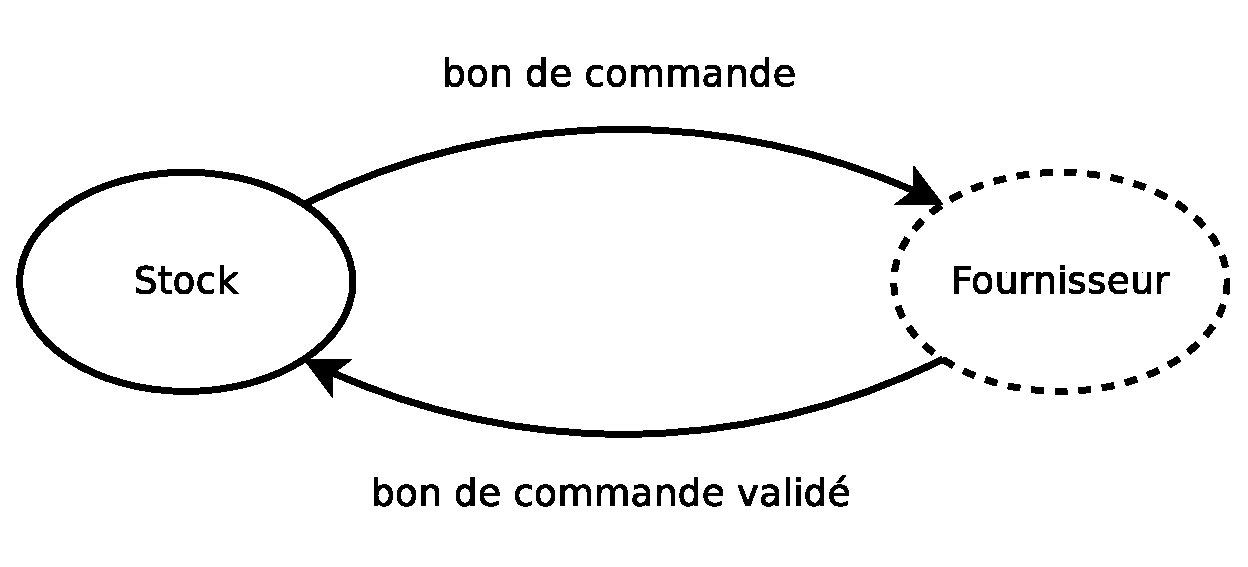
\includegraphics[width=7cm]{images/mcc_commander.eps}
    \caption{\label{mcc_commander} Commander}
    \end{center}
\end{figure}

\begin{figure}[!htb]
    \begin{center}
    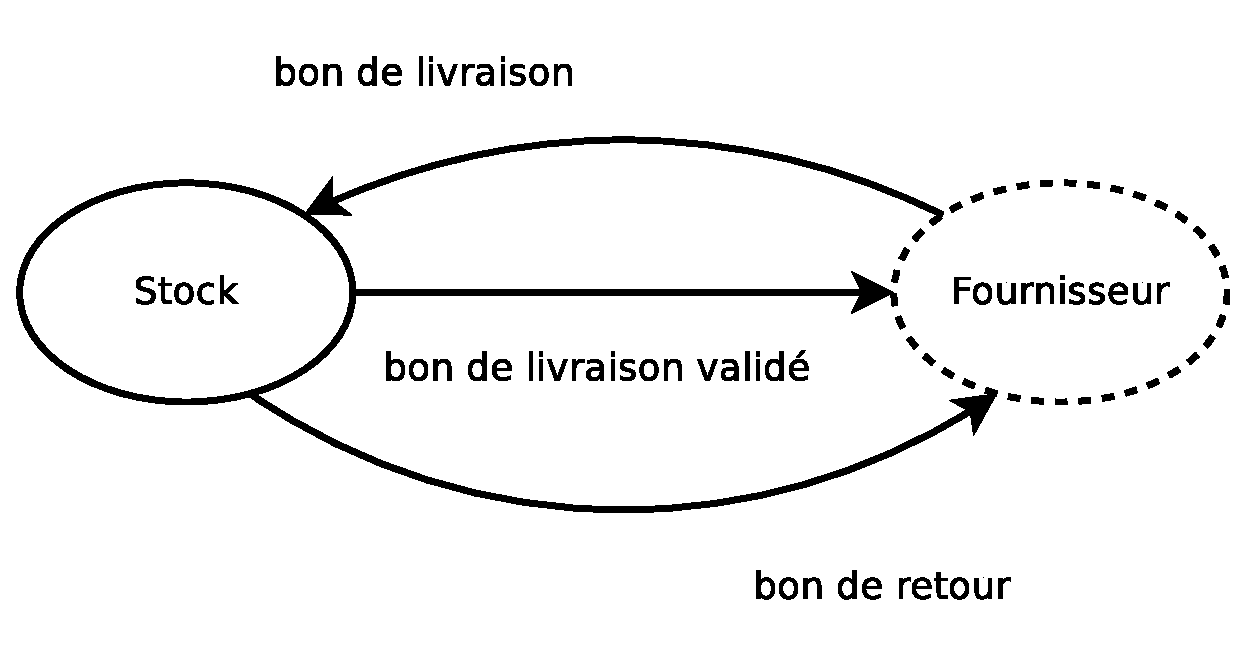
\includegraphics[width=7cm]{images/mcc_livrer.eps}
    \caption{\label{mcc_livrer} Livrer}
    \end{center}
\end{figure}

\begin{figure}[!htb]
    \begin{center}
    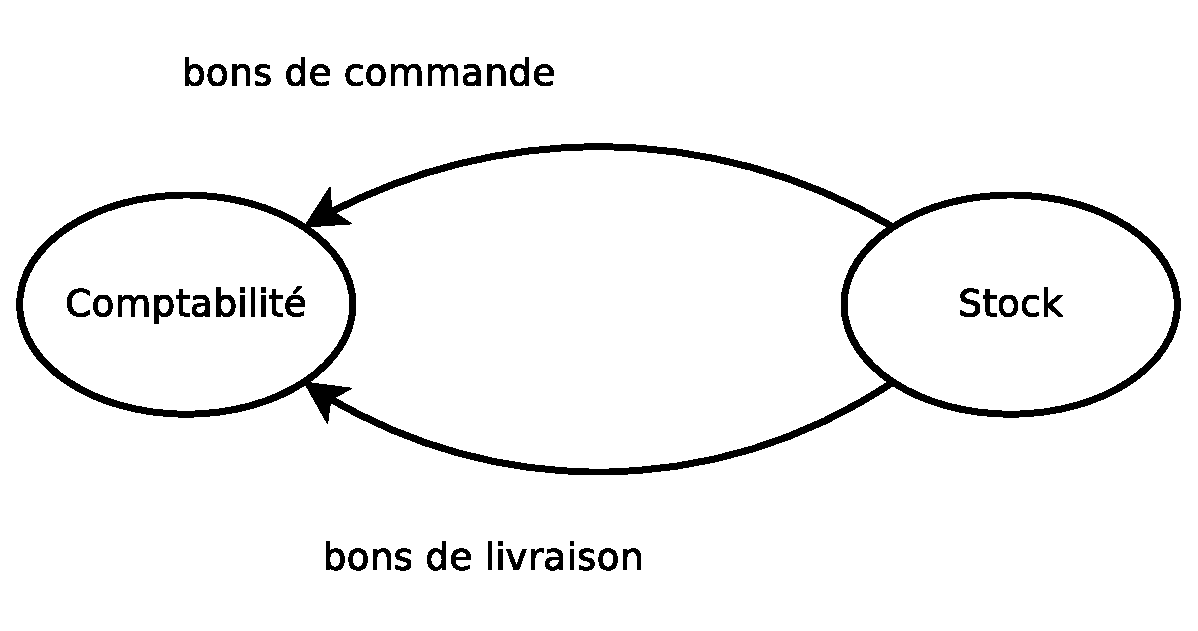
\includegraphics[width=7cm]{images/mcc_al.eps}
    \caption{\label{mcc_al} Avertir de la livraison}
    \end{center}
\end{figure}

\begin{figure}[!htb]
    \begin{center}
    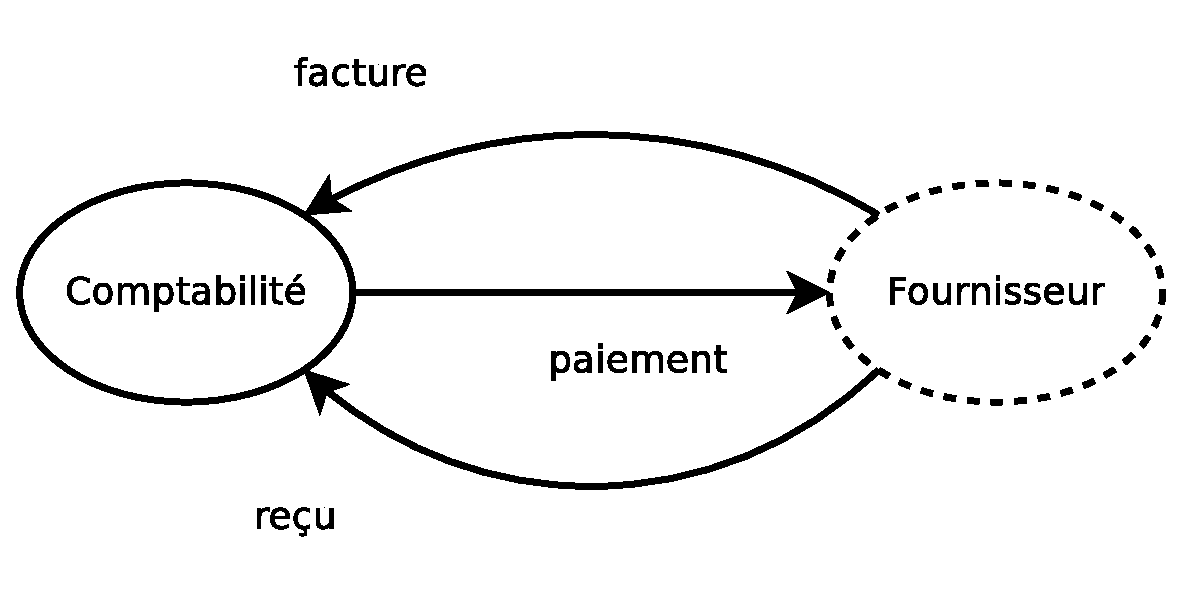
\includegraphics[width=7cm]{images/mcc_payer.eps}
    \caption{\label{mcc_payer} Payer facture}
    \end{center}
\end{figure}

\begin{figure}[!htb]
    \begin{center}
    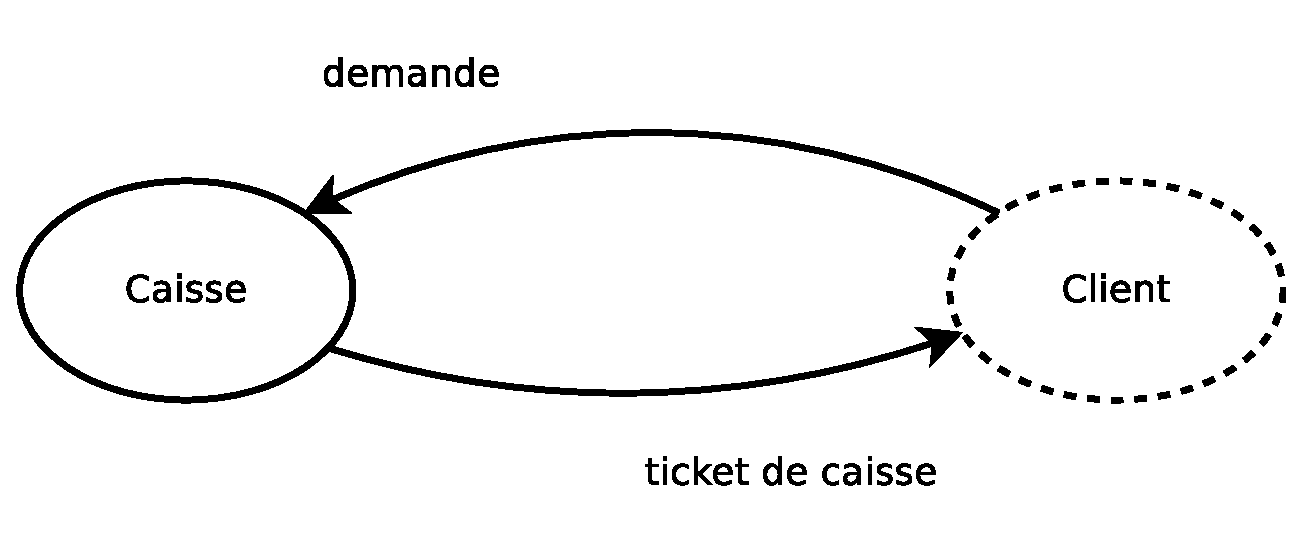
\includegraphics[width=7cm]{images/mcc_acheter.eps}
    \caption{\label{mcc_acheter} Acheter}
    \end{center}
\end{figure}

\begin{figure}[!htb]
    \begin{center}
    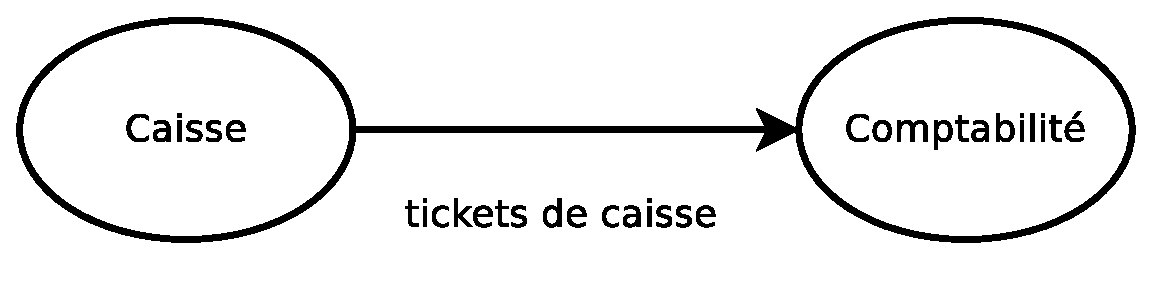
\includegraphics[width=7cm]{images/mcc_isv.eps}
    \caption{\label{mcc_isv} Informer sur les ventes}
    \end{center}
\end{figure}

\begin{figure}[!htb]
    \begin{center}
    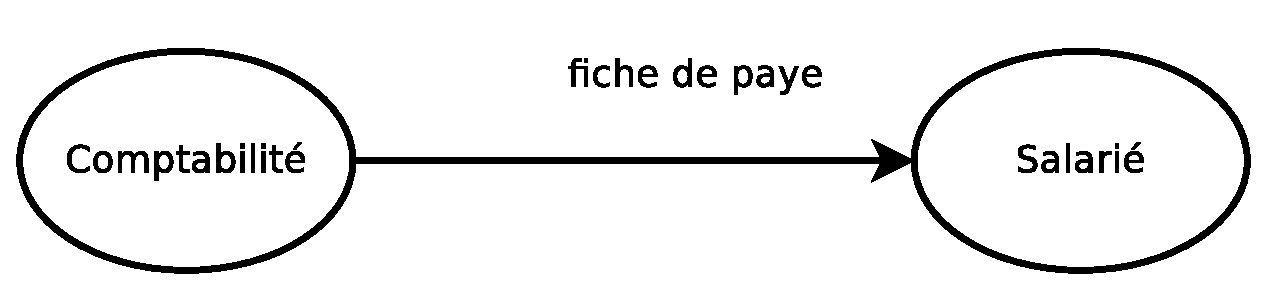
\includegraphics[width=7cm]{images/mcc_ps.eps}
    \caption{\label{mcc_ps} Payer salaire}
    \end{center}
\end{figure}

\begin{figure}[!htb]
    \begin{center}
    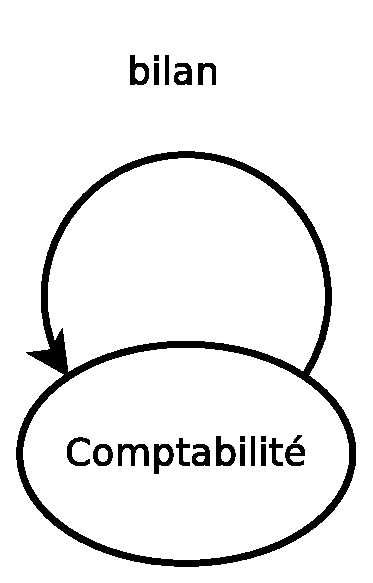
\includegraphics[width=2cm]{images/mcc_bilan.eps}
    \caption{\label{mcc_ps} Faire bilan}
    \end{center}
\end{figure}


\section*{Modèle Concptuel de Communication détaillé}

On place affecte maintenant chaque donnée du dictionnaire de données dans le message qui la contient.

\subsubsection*{bon de commande(Stock, Fournisseur)}
\begin{itemize}
    \item nom-fournisseur
    \item date-commande
    \item ref-commande-fournisseur
    \item adresse-fournisseur
    \item nom-produit-acheté
    \item prix-produit-acheté
    \item quantité-produit-acheté
    \item ref-produit-fournisseur
\end{itemize}

\subsubsection*{bon de commande validé(Fournisseur, Stock)}
\begin{itemize}
    \item nom-fournisseur
    \item ref-commande-fournisseur
\end{itemize}

\subsubsection*{bon de livraison(Fournisseur, Stock)}
\begin{itemize}
    \item nom-fournisseur
    \item date-livraison
    \item ref-bon-livraison-fournisseur
    \item ref-commande-fournisseur
\end{itemize}

\subsubsection*{bon de livraison validé(Stock, Fournisseur)}
\begin{itemize}
    \item nom-fournisseur
    \item adresse-fournisseur
    \item ref-bon-livraison-fournisseur
\end{itemize}

\subsubsection*{bon de retour(Stock, Fournisseur)}
\begin{itemize}
    \item nom-fournisseur
    \item adresse-fournisseur
    \item ref-bon-livraison-fournisseur
    \item date-retour
\end{itemize}

\subsubsection*{bons de commande(Stock, Comptabilité)}
\begin{itemize}
    \item nom-fournisseur
    \item ref-commande-fournisseur
    \item nom-produit-acheté
    \item quantité-produit-acheté
    \item prix-produit-acheté
    \item ref-produit-fournisseur
\end{itemize}

\subsubsection*{bons de livraison(Stock, Comptabilité)}
\begin{itemize}
    \item nom-fournisseur
    \item ref-bon-livraison-fournisseur
    \item ref-commande-fournisseur
\end{itemize}

\subsubsection*{facture(Fournisseur, Comptabilité)}
\begin{itemize}
    \item nom-fournisseur
    \item ref-facture-fournisseur
    \item ref-commande-fournisseur
    \item date-facturation
\end{itemize}

\subsubsection*{paiement(Comptabilité, Fournisseur)}
\begin{itemize}
    \item ref-facture-fournisseur
    \item date-paiement
\end{itemize}

\subsubsection*{reçu(Fournisseur, Comptabilité)}
\begin{itemize}
    \item ref-facture-fournisseur
\end{itemize}

\subsubsection*{demande(Client, Caisse)}
\begin{itemize}
    \item nom-produit-vendu
    \item quantité-produit-vendu
\end{itemize}

\subsubsection*{ticket de caisse(Caisse, Client)}
\begin{itemize}
    \item ref-ticket
    \item date-ticket
    \item nom-produit-vendu
    \item prix-produit-vendu
    \item quantité-produit-vendu
\end{itemize}

\subsubsection*{tickets de caisse(Caisse, Comptabilité)}
\begin{itemize}
    \item ref-ticket
    \item date-ticket
    \item nom-produit-vendu
    \item prix-produit-vendu
    \item quantité-produit-vendu
\end{itemize}

\subsubsection*{fiche de paye(Comptabilité, Employé)}
\begin{itemize}
    \item ref-fiche-paye
    \item date-paye
    \item nom-employé
    \item date-naissance-employé
    \item adresse-employé
    \item salaire-employé
\end{itemize}

\subsubsection*{bilan(Comptabilité, Comptabilité)}
\begin{itemize}
    \item date-début
    \item date-fin
\end{itemize}

\section*{Modèle Conceptuel de Données}

En suivant l'ordre des messages du MCC, on place chaque donnée véhiculée par un message dans le MCD. Pour chaque donnée, on se pose la question de l'existance d'une nouvelle entité. Une fois toutes les données placées, on valide notre MCD (formes normales).

\begin{figure}[!htb]
    \begin{center}
    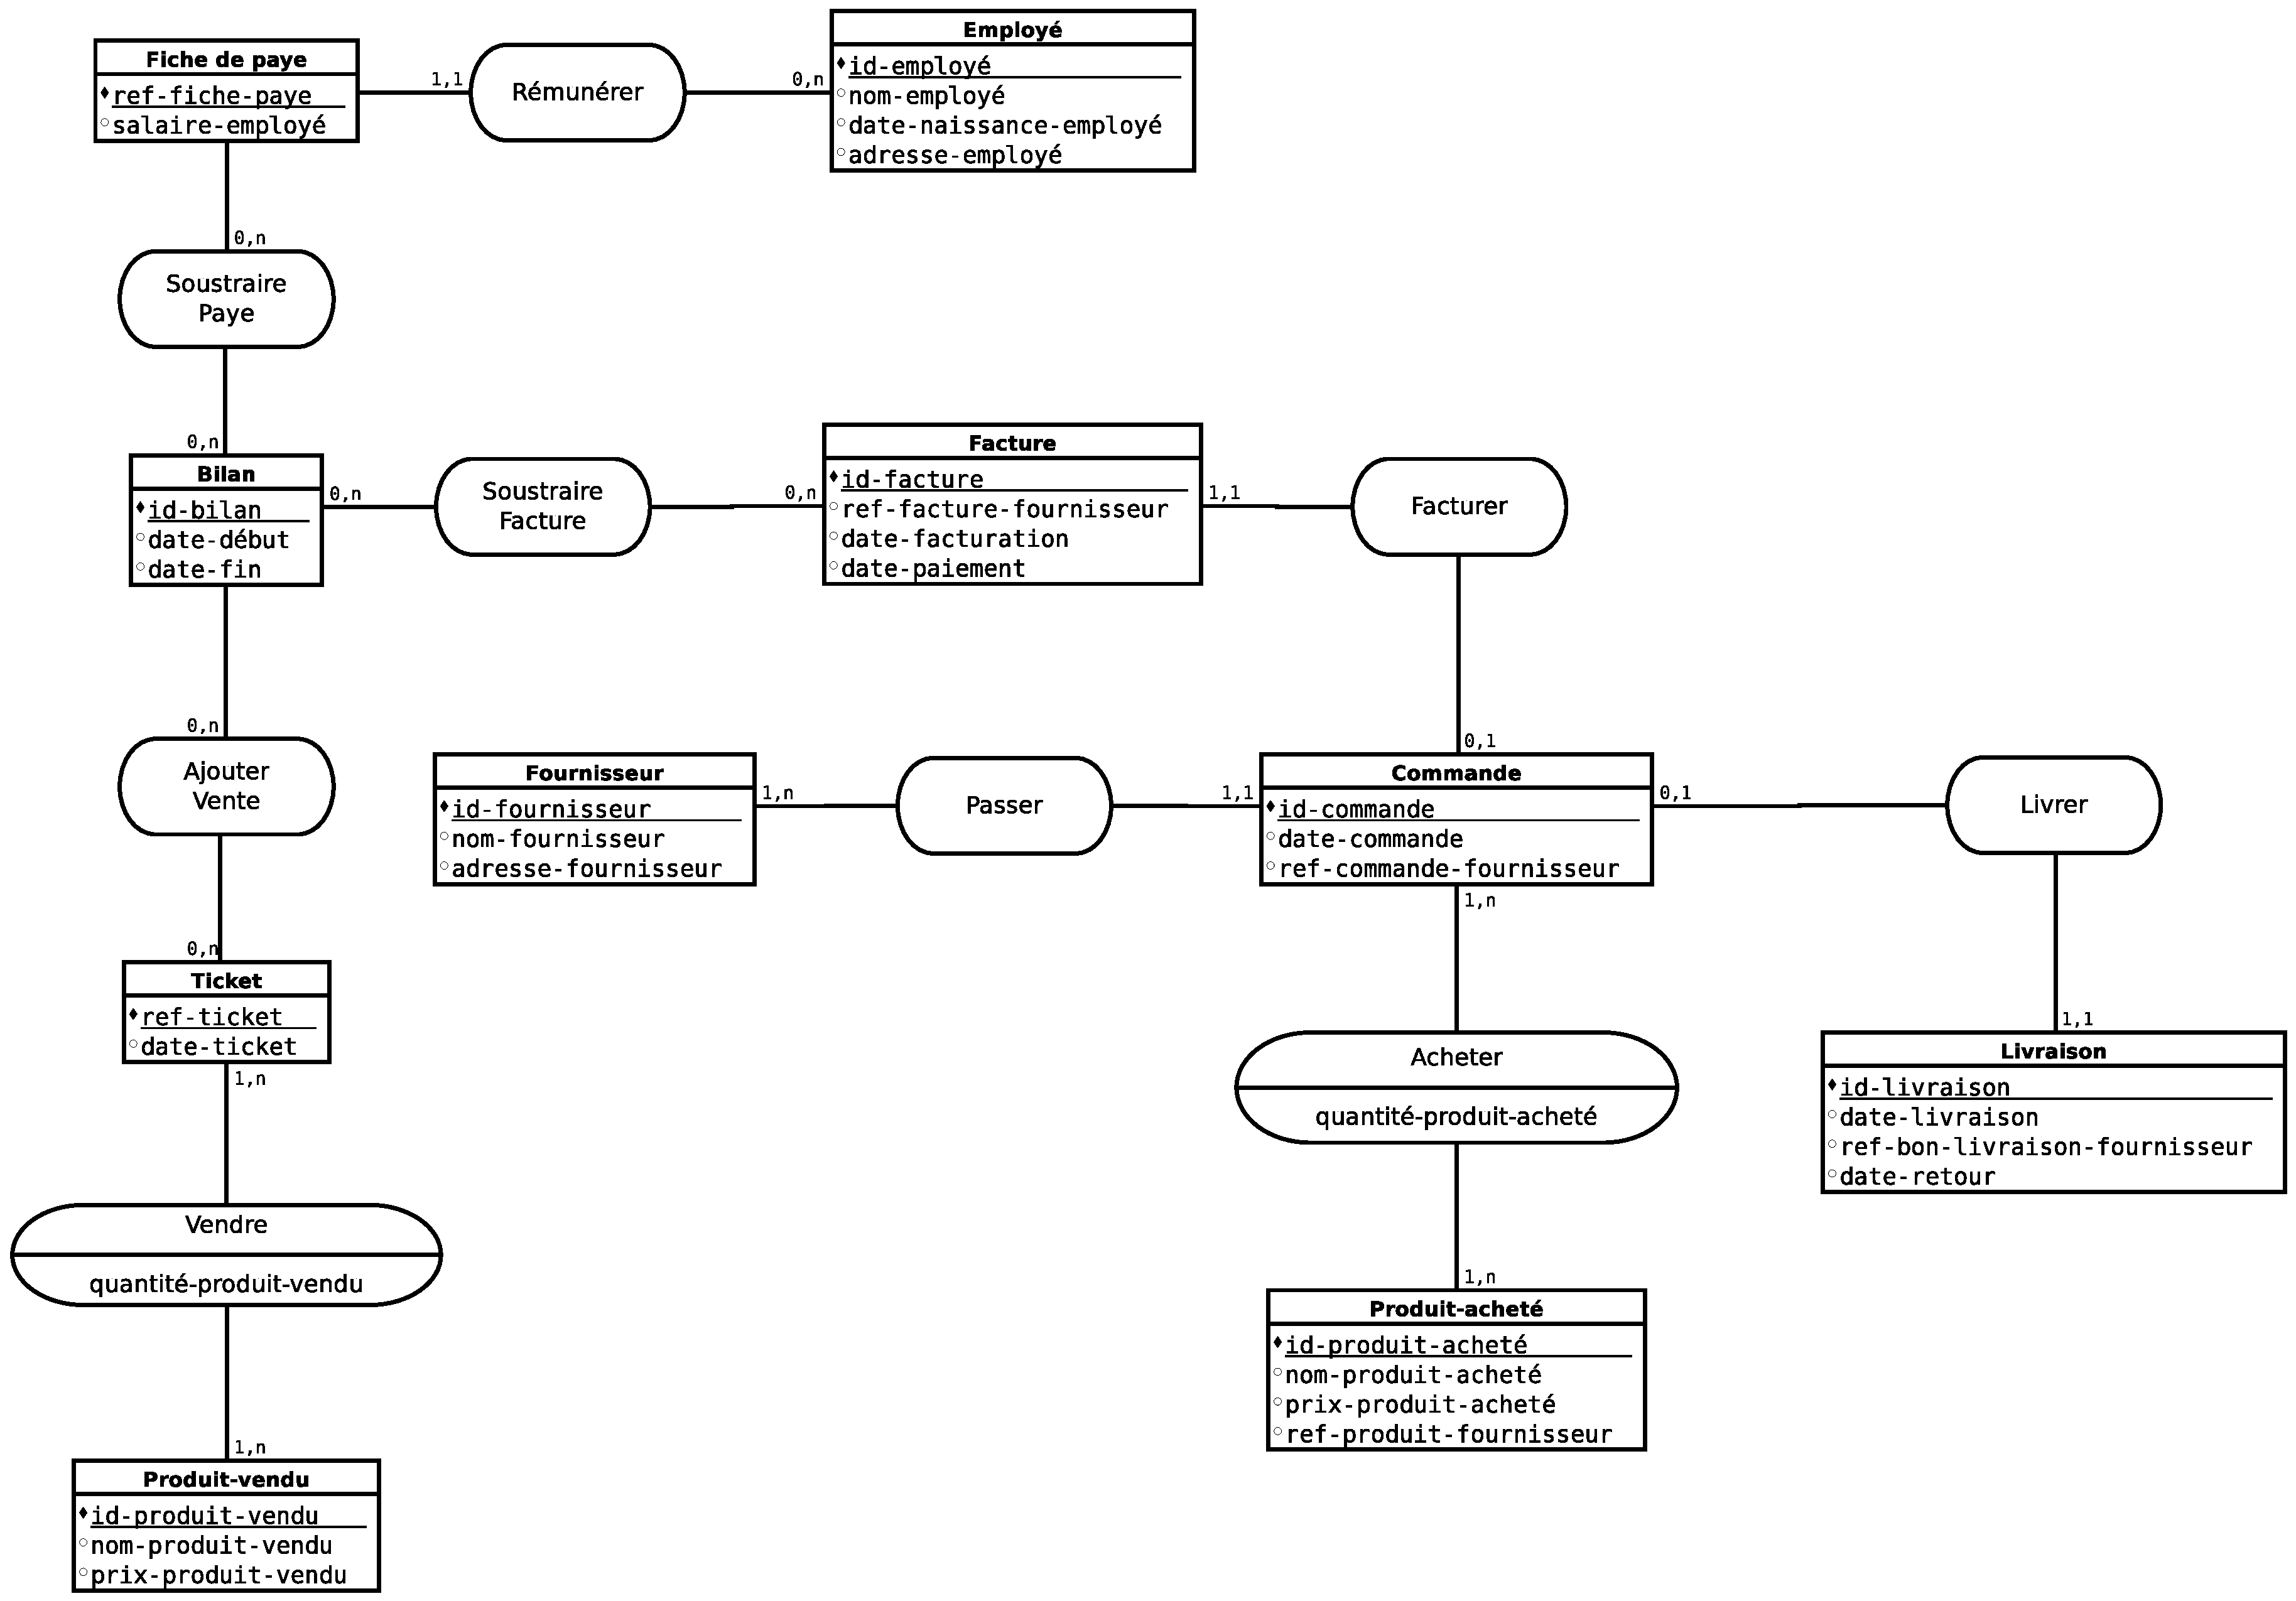
\includegraphics[width=15cm]{images/mcd.eps}
    \caption{\label{mcd} MCD}
    \end{center}
\end{figure}
